\documentclass[a4paper,11pt,oneside]{scrreprt}
\usepackage[latin1]{inputenc}
\usepackage[english]{babel}
\usepackage{graphicx}
\usepackage{float}
\usepackage{geometry}
\geometry{verbose,a4paper,tmargin=25mm,bmargin=25mm,lmargin=15mm,rmargin=25mm}
\usepackage{paralist}

\usepackage{paracol}

\usepackage{todonotes}

\usepackage{listings}
\lstset{language=Java,
	tabsize=2,
	showspaces=false,
	showtabs=false,
	breaklines=true,
	showstringspaces=false,
	breakatwhitespace=true,
	commentstyle=\color{pgreen},
	keywordstyle=\color{pblue},
	stringstyle=\color{pred},
	basicstyle=\footnotesize\ttfamily,
	moredelim=[il][\textcolor{pgrey}]{$$},
	moredelim=[is][\textcolor{pgrey}]{\%\%}{\%\%}
}

\usepackage{tikz}
\usetikzlibrary{calc,patterns,angles,quotes}

\usepackage{caption}
\usepackage{subcaption}
\usepackage{tabularx} % in the preamble
\usepackage{pdfpages}
\usepackage{grffile}

\begin{document}


\begin{center}
	Submitted by Group 36
	
	\bigskip
	
	\begin{tabular}{c}
	Group Members: \\
	CETIN, Ulfet (391819); GRUCZKA, FILIP (413279);	LIPINSKI, Bartosz (413177) \\
	\end{tabular}

	\bigskip
	
	DIS1 WS 19/20 Assignment 2\\
	Applying Design Principles to Evaluate and Redesign UIs
	
	%	(ordered on lastname basis)
\end{center}

\section*{Task 1}

\begin{figure}[H]
	\centering
	
\includegraphics[clip, trim=0cm 0cm 0cm 0cm, scale=0.33]{./images/redesign.png}
	\caption{Blinkee}
	\label{fig:sub3}
\end{figure}

\begin{figure}[H]
	\centering
	
\includegraphics[clip, trim=0cm 0cm 0cm 0cm, scale=0.33]{./images/redesign.png}
	\caption{Blinkee}
	\label{fig:sub2}
\end{figure}

\clearpage


\begin{table}[h]
	\begin{tabularx}{\textwidth}{|X|}
		
		\hline
			\\
			\textbf{Natural Mappings and Forcing Functions: Examples} \\
			\\
		\hline
		
			\textbf{Natural mapping with spatial analogy:}			\\
			placeholder\\
			
		\hline
				
			\textbf{Natural mapping with perceptual analogy:}			\\
			placeholder\\
			
		\hline
		
			\textbf{Natural mapping with cultural analogy:}			\\
			placeholder\\
			
		\hline
		
			\textbf{Forcing function:}			\\
			placeholder\\
			
			\hline
		
		\hline
	\end{tabularx}
\end{table}

\clearpage

\section*{Task 2}

\begin{figure}[H]
	\centering
	
\includegraphics[clip, trim=0cm 0cm 0cm 0cm, scale=0.33]{./images/redesign.png}
	\caption{Home Appliance Picture for Task 2}
	\label{fig:sub4}
\end{figure}

\textbf{Task Description:}
\clearpage

% this is how one adds a PDF file into LaTex
% 	please do not annotate the submission file
%		instead, annotate another pdf file, then import using the following command
\includepdf[scale=1.0,pages=4-4,clip,trim=0cm 2cm 0cm 4cm, pagecommand={}]{../format.pdf}

\section*{Task 3}

\textbf{Example of a home appliance more closely associated with level **********:}

\begin{figure}[H]
	\centering
	
\includegraphics[clip, trim=0cm 0cm 0cm 0cm, scale=0.33]{./images/redesign.png}
	\caption{Placeholder Image for Ex1}
\end{figure}

\noindent Justification:\\
placeholder

\vspace{5mm}

\textbf{Example of a home appliance more closely associated with level **********:}

\begin{figure}[H]
	\centering
	
\includegraphics[clip, trim=0cm 0cm 0cm 0cm, scale=0.33]{./images/redesign.png}
	\caption{Placeholder Image for Ex1}
\end{figure}

\noindent Justification:\\
placeholder

\vspace{5mm}

\textbf{Example of a home appliance more closely associated with level **********:}

\begin{figure}[H]
	\centering
	
\includegraphics[clip, trim=0cm 0cm 0cm 0cm, scale=0.33]{./images/redesign.png}
	\caption{Placeholder Image for Ex1}
\end{figure}

\noindent Justification:\\
placeholder


\end{document}
